% !TEX root = FDS_Technical_Reference_Guide.tex

% \usepackage{tikz,tikz-3dplot}
% \usetikzlibrary{arrows}

% \newenvironment{myfont}{\fontfamily{\ttdefault}\selectfont}{\par}

% \mathchardef\mhyphen="2D


\typeout{new file: Wildland_Chapter.tex}


\chapter{Wildland Fire Spread}
\label{sec:wildland_spread}

\section{Particle Model}

In the case that vegetation is represented using Lagrangian particles to capture the details of vegetation heat transfer and thermal decomposition, details of the technical approach can be found in other sections of this guide. This approach makes use of the general models for particle drag, particle radiation attenuation and emission, and thermal decomposition, with additional detail to be found in the relevant sections.

\section{Level Set Model}

This method allows the details of heat transfer and vegetation decomposition to be parameterized with an empirical spread rate function, greatly reducing the complexity of the model. In general, the level set method represents an interface (in this case a fire front) using a continuous scalar function, denoted as $\phi(\mathbf{x},t)$. The zero-level of this function, $\phi(\mathbf{x},t)=0$, defines the position of the interface. The function is initialized with values that are negative on the unburned side of the interface and positive on the other, allowing it to evolve over time as the fire spreads. The rate of change at a given point can be written as
\begin{equation}
\frac{d\phi}{dt} = \frac{\partial\phi}{\partial t} + \frac{\partial\phi}{\partial x}\frac{dx}{dt} + \frac{\partial\phi}{\partial y}\frac{dy}{dt} = 0
\end{equation}
The terms $\frac{dx}{dt}$ and $\frac{dy}{dt}$ can be replaced by the front spread rates $R_x$ and $R_y$.
\begin{equation}
\frac{\partial\phi}{\partial t} + R_x\frac{\partial\phi}{\partial x} + R_y\frac{\partial\phi}{\partial y} = 0
\label{eq:level_set}
\end{equation}


\subsection{Richards Elliptical Model}

As described in Bova~\textit{et al.}~\cite{Bova:IJWF2015} the default formulation in FDS determines the spread rates $R_x$ and $R_y$ by assuming a fire spreading from each point along the front with an elliptical shape and a fixed length-to-breadth ratio~\cite{Richards:1990}. Using this description, the head, flank, and back fire spread rates for an ellipse are written as $b+c$, $a$, and $b-c$, respectively. In terms of geometry, $a$ is the semi-minor axis of the ellipse, $b$ is the semi-major axis of the ellipse, and $c$ is the distance between the initial point and the center of the ellipse. The ellipse grows in the maximum spread direction, $\theta$, which is based on the wind and slope vectors and is in compass notation (clockwise from positive $y$-axis). The components of the spread rate at a point along the front, to be used in Eq.~\ref{eq:level_set}, can then be written as
\begin{equation}
R_{x} = D\left[a^{2} \, \cos \theta\left(x_{s}\, \sin \theta+y_{s} \cos \, \theta\right)-b^{2} \,\sin \theta\left(x_{s} \,\cos \theta - 
y_{s} \, \sin \theta\right)\right]+ c \, \sin \theta
\end{equation}
\begin{equation}
R_{y} = D\left[-a^{2} \, \sin \theta\left(x_{s} \, \sin \theta+y_{s} \, \cos \theta\right)-b^{2} \, \cos \theta\left(x_{s} \, \cos \theta - 
y_{s} \, \sin \theta\right)\right]+c \, \cos \theta
\end{equation}
where the denominator, $D$, is
\begin{equation}
D = \left[a^{2}\left(x_{s} \, \sin \theta+y_{s} \, \cos \theta\right)^{2}+b^{2}\left(x_{s} \, \cos \theta-y_{s} \, \sin \theta\right)^{2}\right]^{-\frac{1}{2}}
\end{equation}
The vector $(x_s,y_s)$ is the differential along the path of the ellipse and is related to the normal of the fireline (level set function) by
\begin{equation}
(x_s,y_s) = \left(\frac{\partial\phi}{\partial y}, -\frac{\partial\phi}{\partial x} \right)
\end{equation}
To solve the above equations, we then require the head, back, and flank fire spread rates. The current implementation in FDS follows that originally employed in FARSITE~\cite{Finney:FARSITE}. The length-to-breadth ratio of the ellipse, $L B$, is determined by the virtual wind speed $U$, bounded by some limiting values
\begin{gather}
L B=0.936 \, \exp (0.2566 \, U)+0.461 \, \exp (-0.1548 \, U)-0.397 \\[8pt]
L B=\max (1, \min (L B, 8))
\end{gather}
Using an intermediary value, the head-to-backing spread ratio, $H B$, the necessary elliptical spread parameters can then be calculated based on a head fire spread rate, $R$
\begin{gather}
H B = \left(L B+\sqrt{L B^{2}-1}\right) /\left(L B-\sqrt{L B^{2}-1}\right) \\[8pt]
a = \frac{b}{L B} \\[8pt]
b = \frac{1}{2}\left(R+\frac{R}{H B}\right) \\[8pt]
c = b-\frac{R}{H B}
\end{gather}
Following Finney~\cite{Finney:FARSITE}, the above wind speed is referred to as ``virtual'' as it includes both wind and slope effects on the elliptical growth. This wind speed is the vector sum of the true wind speed at midflame height, $\mathbf{U}_{\rm mf}$, and a second vector that represents an equivalent wind that would reproduce any slope effects, $\mathbf{U}_{\rm s}$ 
\begin{equation}
\mathbf{U} = \mathbf{U}_{\rm mf} + \mathbf{U}_{\rm s}
\end{equation}
This not only determines the shape of the ellipse, based on the magnitude of $\mathbf{U}$, but the direction of maximum spread, $\theta$. This approach then provides spread rates along the surface of the slope, $R_{x'}$ and $R_{y'}$. Equation~\ref{eq:level_set}, on the other hand, considers the projection of the fireline onto the horizontal plane. Therefore the spread rates used in Eq.~\ref{eq:level_set} are scaled based on the slope, $\left(\frac{\partial z}{\partial x},\frac{\partial z}{\partial y}\right)$, as
\begin{gather}
R_x = R_{x'} \, \cos \left(\arctan \left(\frac{\partial z}{\partial x}\right)\right) \\[8pt]
R_y = R_{y'} \, \cos \left(\arctan \left(\frac{\partial z}{\partial y}\right)\right) \\[8pt]
\end{gather}

\subsection{Rothermel Spread Model}

The above formulation uses the elliptical growth model to solve the two-dimensional evolution of a fire front based on a head fire spread rate, $R$. However, it does not define what this spread rate is and how it varies as a function of fuel properties, wind speed, and slope. There are a number of ways to define and customize these relationships, as described in the User's Guide, but the default approach uses the Rothermel~\cite{Rothermel:1972,Albini:1976} formulae. 

There are effectively two components to the Rothermel model. The first component is the no-wind, no-slope value of spread rate, $R_0$. The Rothermel model presents this spread rate as a ratio between energy received by an unburnt fuel package and the energy required for ignition. These terms are formulated as empirical functions of fuel bed properties. In FDS, the 13 fuel models introduced by Rothermel and Albini~\cite{Rothermel:1972,Albini:1976} are available. The calculation procedure for obtaining $R_0$ from the fuel model properties follows that outlined in numerous other references (e.g.~\cite{Rothermel:1972,Wilson:1980}) and is not repeated here. However, this model can also be overridden with a user-supplied $R_0$.

The second component of the model is the inclusion of wind and slope effects on the head fire spread rate. These are introduced with parameters $\phi_{\rm W}$ and $\phi_{\rm S}$, respectively (note that these have nothing to do with the level set value $\phi$, but the nomenclature is adopted for consistency with the original notation). The wind speed function, $\phi_{\rm W}$, depends on fuel properties (surface-to-volume ratio, $\sigma$; packing ratio, $\beta$; optimum packing ratio, $\beta_{\rm op}$) and takes the following form
\begin{gather}
\phi_{\rm W} = C\left(3.281 \, U_{\rm mf}\right)^{B}\left(\frac{\beta}{\beta_{\rm op}}\right)^{-E} 
\label{eq:roth_wind} \\[8pt]
B = 0.15988 \, \sigma^{0.54} \\[8pt]
C = 7.47 \, \exp \left(-0.8711 \, \sigma^{0.55}\right) \\[8pt]
E = 0.715 \, \exp (-0.01094 \, \sigma) \\[8pt]
\beta_{\text {op }} = 0.20395 \, \sigma^{-0.8189}
\end{gather}
However, this can also be defined as a custom function using \ct{RAMP} functionality. The slope function, $\phi_{\rm W}$, is defined as
\begin{equation}
\phi_{\rm S} = 5.275 \, \beta^{-0.3}(\tan \Phi)^{2} \label{eq:roth_slope}
\end{equation}
where $\Phi$ is the slope angle

In the original Rothermel model, these effects are considered only in the case that wind and slope are aligned with the direction of fire spread~\cite{Rothermel:1972}. In this way, the effect on the head fire spread rate can be written as
\begin{equation}
R = R_0 \, (1+ \phi_{\rm W} + \phi_{\rm S})
\end{equation}
To extend this to two dimensions, we need to consider that the slope and wind may not be aligned. Therefore, these factors are treated as vectors, $(\phi_{\mathrm{W},x}, \phi_{\mathrm{W},y})$ and $(\phi_{\mathrm{S},x}, \phi_{\mathrm{S},y})$, and the effect on head fire spread rate comes from the vector sum
\begin{equation}
R = R_0 \, \left(1 + \sqrt{(\phi_{\mathrm{W},x} + \phi_{\mathrm{S},x})^2 + (\phi_{\mathrm{W},y} + \phi_{\mathrm{S},y})^2}\right)
\end{equation}
The vector form of the wind factor is based on the direction of the midflame wind speed
\begin{equation}
(\phi_{\mathrm{W},x}, \phi_{\mathrm{W},y}) = 
C \left(3.281 \, U_{\rm mf}\right)^{B-1}\left(\frac{\beta}{\beta_{\rm op}}\right)^{-E} \, (U_{\rm mf,x},U_{\rm mf,y})
\end{equation}
and the vector form of the slope factor is based on the direction of the gradient vector
\begin{equation}
(\phi_{\mathrm{S},x}, \phi_{\mathrm{S},y}) = 
5.275 \, \beta^{-0.3} \, \tan \Phi \left(\frac{dz}{dx},\frac{dz}{dy}\right)
\end{equation}
Note that the vector forms of these factors differ slightly from those presented in Bova~\textit{et al.}~\cite{Bova:IJWF2015}. They have been adjusted to ensure that their magnitudes are always matched to the original form presented by Rothermel~\cite{Rothermel:1972}.

As mentioned above, to include the effect of slope in the elliptical growth model an equivalent virtual wind vector should be calculated. Combining Eq.~\ref{eq:roth_wind} and Eq.~\ref{eq:roth_slope}, the magnitude of this virtual wind is
\begin{equation}
U_{\rm s} = 0.3048\left[\frac{\phi_{\rm S}}{C}\left(\frac{\beta}{\beta_{\mathrm{op}}}\right)^{E} 
\right]^{\frac{1}{B}}
\end{equation}
As a vector, this virtual wind acts in the direction of the slope
\begin{equation}
\mathbf{U}_{\rm s} = \frac{U_{\rm s}}{\phi_{\rm S}} \left(\phi_{\mathrm{S},x},\phi_{\mathrm{S},y}\right)
\end{equation}

\subsection{Midflame Wind Speed}

Both the elliptical growth model for two-dimensional spread and the Rothermel model for determining the maximum spread rate assume a reference wind speed at ``midflame'' height. This is not trivial to define and the default approach in FDS is to copy the assumption made in common operational fire models. This assumption is that the midflame height is one fuel bed height above the top of the fuel. Further, the wind speed at this height is inferred by assuming a logarithmic flow profile and sampling a reference wind speed, $\mathbf{U}_{\rm ref}$, at 6.1~m above the ground (equivalent to a standard 20~ft weather station measurement)~\cite{Andrews:2012}. The wind speed is then calculated as
\begin{equation}
\mathbf{U}_{\rm mf}=\mathbf{U}_{\rm ref} \frac{1.83}{\ln \left(\frac{20+1.18 h}{0.43 h}\right)}
\end{equation}
This re-scaling procedure is typically referred to as a Wind Adjustment Factor (WAF). However, in FDS it may be the case that the near-surface winds are relatively well resolved, and these basic assumptions may not match the actual flow field. Therefore, it is also possible to specify a custom reference wind height for a given fuel surface. In this case the flow field is directly sampled at the specified height with no adjustment factor.

\subsection{Numerical Method}

To solve Eq.~\ref{eq:level_set} on the FDS grid, the gradients of the level set value, $\phi$, at location $(i,j)$ and time step $n$ are approximated using a flux-limiting scheme. A central difference is computed based on estimated values of $\phi$ at the cell faces (noted with $\frac{1}{2}$ subscript)
\begin{gather}
\left(\frac{\partial \phi}{\partial x}\right)_{i, j}^{n} \approx \left(\frac{\delta \phi}{\delta x}\right)_{i, j}^{n} =
\frac{\phi_{i+\frac{1}{2}, j}^{n}-\phi_{i-\frac{1}{2}, j}^{n}}{\Delta x} \\[8pt]
\left(\frac{\partial \phi}{\partial y}\right)_{i, j}^{n} \approx \left(\frac{\delta \phi}{\delta y}\right)_{i, j}^{n} =
\frac{\phi_{i, j+\frac{1}{2}}^{n}-\phi_{i, j-\frac{1}{2}}^{n}}{\Delta y}
\end{gather}
The face values depend on the ratio of local to upwind difference in $\phi$
\begin{equation}
r= \begin{cases}
    \frac{\Delta \phi_{\rm upwind}}{\Delta \phi_{\rm local}} & \phi_{\rm local} \neq 0 \\[6pt]
    0 & \phi_{\rm local} = 0
\end{cases}
\end{equation}
If we take the example of the face $i+\frac{1}{2}$ then
\begin{gather}
\phi_{\rm local} = \phi_{i+1, j}-\phi_{i, j}
\phi_{\rm upwind}= \begin{cases}
    \phi_{i, j}-\phi_{i-1, j} &  \quad R_x > 0 \\[6pt]
    \phi_{i+2, j}-\phi_{i+1, j} & \quad R_x < 0
\end{cases}
\end{gather}
and the level set value is computed as
\begin{equation}
\phi_{i+\frac{1}{2},j} = \phi_{i,j} + 0.5 \, B(r) \left[\phi_{i+1,j}-\phi_{i,j} \right]
\end{equation}
The value of $B(r)$ depends on the choice of flux-limiting scheme
\begin{equation}
B(r)= \begin{cases}
    0 & \mathrm{Godunov} \\[4pt]
    \max(0, \min(1,r)) & \mathrm{Minmod} \\[4pt]
    \max(0, \min(2,r), \min(1,2r)) & \mathrm{Superbee}
\end{cases}
\end{equation}
Time integration uses the predictor-corrector scheme
\begin{eqnarray}
\phi_{i, j}^{*} &=& \phi_{i, j}^{n}-\left(R_{x} \frac{\delta \phi}{\delta x}+R_{y} \frac{\delta \phi}{\delta y}\right) \Delta t \\[8pt]
\phi_{i, j}^{n+1} &=& \frac{1}{2} \phi_{i, j}^{n}+\frac{1}{2}\left[\phi_{i, j}^{*}-\left(R_{x} \frac{\delta \phi^{*}}{\delta x}+R_{y} \frac{\delta \phi^{*}}{\delta y}\right) \Delta t\right]
\end{eqnarray}
The calculation of the slope uses a central difference of the elevation
\begin{gather}
\left(\frac{\partial z}{\partial x}\right)_{i, j} \approx \left(\frac{\delta z}{\delta x}\right)_{i, j} =
\frac{z_{i+1, j}-z_{i-1, j}}{2 \Delta x} \\[6pt]
\left(\frac{\partial z}{\partial y}\right)_{i, j} \approx \left(\frac{\delta z}{\delta y}\right)_{i, j} =
\frac{z_{i, j+1}-z_{i, j-1}}{2 \Delta y} \\[6pt]
\end{gather}


\subsection{Burning Rate Model}

The level set implementation in FDS includes a mode where the the fire is coupled with the wind field (\ct{LEVEL_SET_MODE=4}). This is done by injecting fuel vapor at burning surfaces following a prescribed rate and allowing gas-phase combustion to occur. The associated energy release leads to buoyancy effects that generate a plume which interacts with the surrounding atmosphere. This mode can be considered similar to the approach in other coupled fire-atmosphere models.

When the fire line reaches a given grid cell ($\phi(\mathbf{x},t)=0$) the prescribed burning rate is determined by the mass of fuel available to burn in the gas-phase
\be
   m_{\rm fv}'' = (1-\nu_{\rm char}) m_{\rm f}''
\ee
Here, $m_{\rm f}''$ is the dry fuel loading in units of kg/m$^2$ and $\nu_{\rm char}$ is the char fraction. The burning duration of a differential area of fuel is assumed to follow the observation of Albini~\cite{Albini:1976} that the dominant parameter is the characteristic surface-to-volume ratio, $\sigma$ (1/m) 
\be
	\delta t = \frac{75600}{\sigma}
\ee
This can be superseded by a user-defined value per fuel surface, if desired.

To compute the burning of a grid cell, it is recognized that the area of the cell does not immediately become fully involved, due to the spreading nature of the fire. Instead, we assume a trapezoidal form to the HRR curve as shown in Fig.~\ref{fig:LS_burning_rate}. The characteristic times $\tau_1$ and $\tau_3$ correspond to the spread rate of the leading edge and trailing edge of the fire, and we assume $\tau_3 = \tau_1$. There are two scenarios which can occur, as shown in Fig.~\ref{fig:LS_burning_rate}, based on the fire depth and grid resolution. The first is that the trailing edge of fire enters the grid cell before the leading edge has crossed the cell (the fire depth is under resolved by the grid). The second is that the trailing edge of the fire does not enter a grid cell for some time {\it after} the leading edge has crossed the entire cell (the fire depth is resolved over multiple grid cells).

\begin{figure}
    \begin{center}
        \scalebox{0.6}{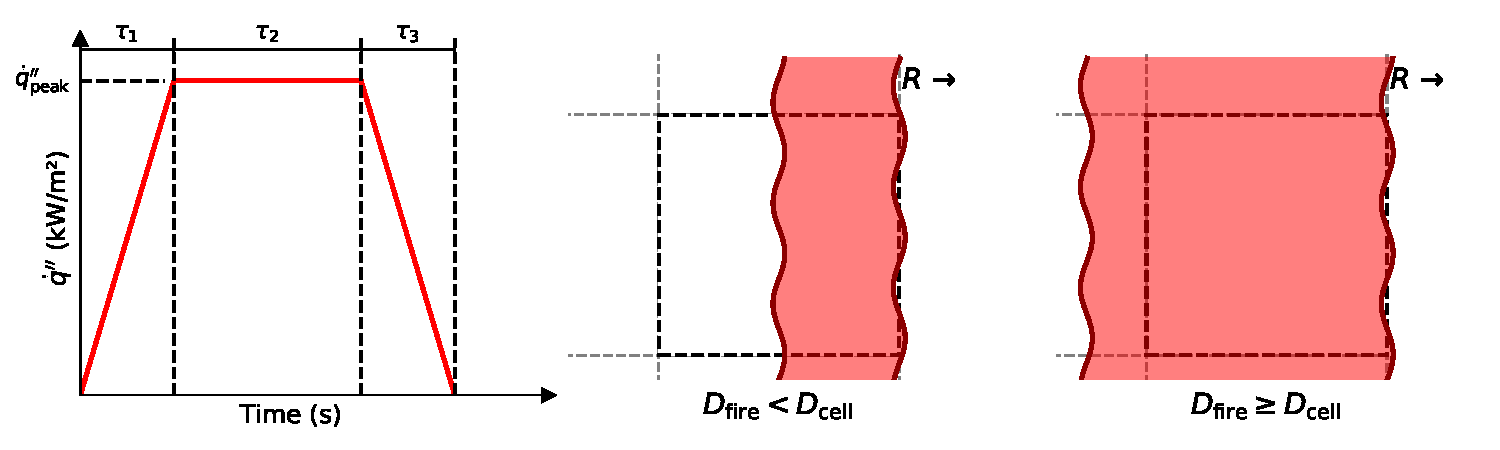
\includegraphics{FIGURES/LS_burning_rate}}
        \caption[Determination of burning rate for cell ignited in level set spread]{\label{fig:LS_burning_rate} Determination of burning rate for cell ignited in level set spread. The heat release per unit area is ramped up linearly, held at a fixed value, and ramped down linearly. The values which define this trapezoidal shape are determined for two possible scenarios. The characteristic cell depth, $D_{\rm cell}$, is greater than the fire depth, $D_{\rm fire}$, or vice versa.}
    \end{center}
\end{figure}

The fire depth is determined from the spread rate as
\begin{equation}
D_{\rm fire} =  R \, \delta t
\end{equation}
and the characteristic cell size is taken as the crossing distance of the fire front (i.e. it depends upon the direction of spread)
\begin{equation}
D_{\rm cell} = \sqrt{\min \left(\Delta x, \; \left|\frac{R_x}{R_y}\right| \, \Delta y \right)^2 + 
\min \left(\Delta y, \; \left|\frac{R_y}{R_x}\right| \; \Delta x \right)^2}
\end{equation}
The ratio of these distances determines the time constants of the trapezoidal burning rate function
\begin{equation}
\tau_1 = \tau_3 = 
\begin{cases}
    \frac{D_{\rm fire}}{R} &  \quad D_{\rm fire} < D_{\rm cell} \\[6pt]
    \frac{D_{\rm cell}}{R} &  \quad D_{\rm fire} \ge D_{\rm cell}
\end{cases}
\end{equation}
\begin{equation}
\tau_2 = 
\begin{cases}
    \frac{D_{\rm cell} - D_{\rm fire}}{R} &  \quad D_{\rm fire} < D_{\rm cell} \\[6pt]
    \frac{D_{\rm fire} - D_{\rm cell}}{R} &  \quad D_{\rm fire} \ge D_{\rm cell}
\end{cases}
\end{equation}
The final constraint is that the total energy released, based on the area of the trapezoid, matches the available energy in the cell
\begin{equation}
\int \dot{q}'' \, dt = \dot{q}_{\rm peak}'' \frac{\tau_1 + 2\tau_2 + \tau_3}{2} = m_{\rm fv}'' \, \Delta H_{\rm c}
\end{equation}
which can be simplified to obtain the peak heat release rate per unit area 
\begin{equation}
\dot{q}_{\rm peak}'' = \frac{m_{\rm fv}'' \, \Delta H_{\rm c}}{\tau_1 + \tau_2}
\end{equation}

